\section{Approach \& Uniqueness}

In order to enforce reservations while still running best effort jobs
opportunistically, our approach is use priority scheduling.

Enforcing priorities requires fewer global runqueue searches than weights do,
because they only need to happen on \textit{class boundary crossings}: on
\exit{}, when a core switches to running lower class processes after having
previously been running high class, and on \entry{}, when a core enqueues a
higher class process. These checks ensure that if a core $c$ is currently
running a BE thread $t$, the scheduler knows that there are no queued and
waiting LC threads anywhere on the machine. If there is a queued LC thread on a
different core $c'$ when $c$ starts running $t$, the \exit{} check, that looks
at every cores' runqueue, will see and steal it. If a new LC thread wakes up on
a different core while $t$ is running, the \entry{} check ensures that $c'$ will
look at $c$'s runqueue, see that it is running a BE thread, and will send the
new LC thread to $c$ via an interrupt, where the interrupt handler will trigger
a scheduling that interrupts $t$.

\begin{figure}[t]
    \centering
    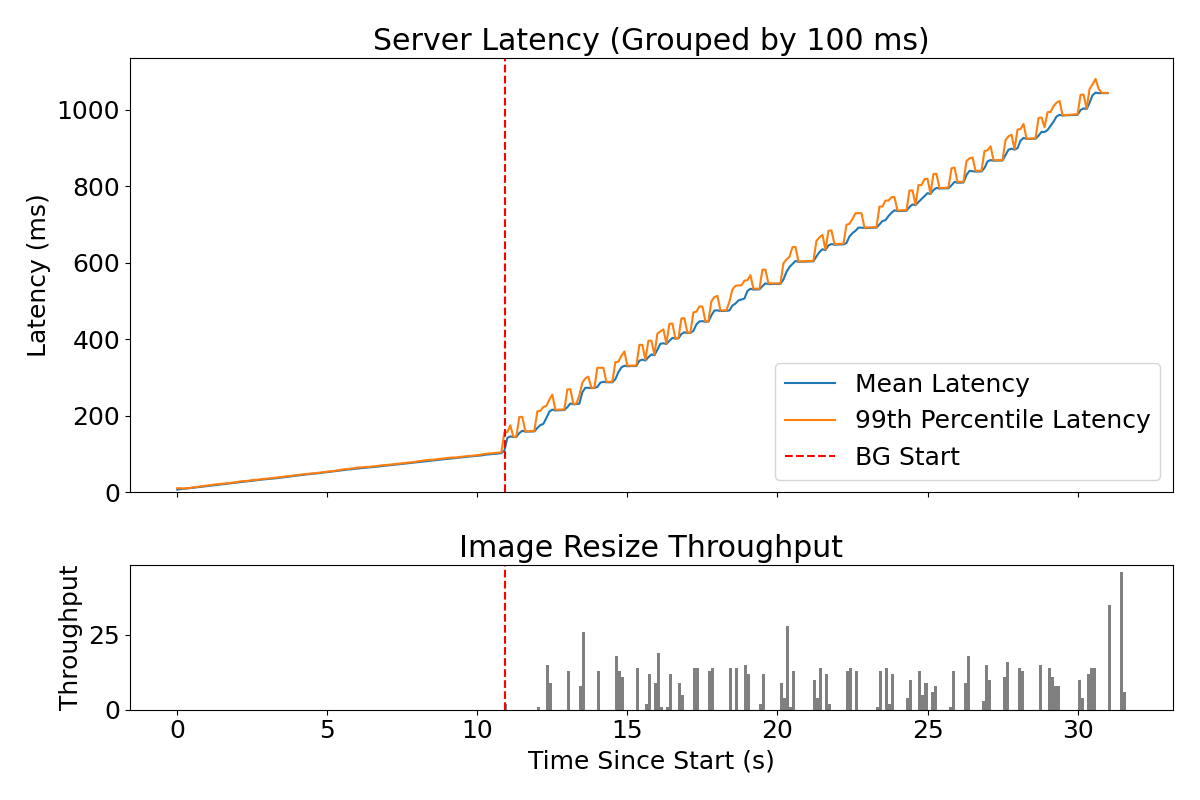
\includegraphics[width=\columnwidth]{graphs/overload-rt.png}
    \caption{LC in real time, throttling}\label{fig:overload-rt}
\end{figure}


Linux already provides priority scheduling across scheduling classes, which are
used to separate real-time applications from all other workload. The priority
scheduling between real-time and the default scheduling classes comes with an
asterisk: if real-time applications experience high load, Linux throttles them
in order to not starve the default class. We can see the result in
\autoref{fig:overload-rt}, where throttling leads to spikes in the background
task as it is able to run, and corresponding spikes in the server's latency.

We design a new scheduling class \beclass{} that sits at a lower priority than
\normalclass{}, which enforces LC applications' uncontended access to the CPUs
they reserved. To enforce reservations even under high load, without throttling
the latency critical services or killing the best effort ones, \beclass{}
\textit{parks} best effort processes. Parking addresses the potential issues
with starvation by separating \beclass{} processes' logic into application logic
(user-space) and critical-state management (kernel-space). When load spikes to
100\%, \beclass{} processes' run only kernel-level services.